\chapter{Sistema Operativo}

\section{Introducción}

Un sistema de cómputo está compuesto de uno o más procesadores, una memoria
principal, discos, interfaces de red y otros dispositivos de entrada/salida. Al
ser un sistema complejo es necesario contar con una capa de \emph{software}
llamada sistema operativo, cuya labor es administrar todos los dispositivos y
proporcionar a los programas de usuario una interfaz sencilla para comunicarse
con el \emph{hardware}\cite{tanenbaum}.

Un sistema operativo puede definirse entonces como un conjunto de programas,
escrito en uno o más lenguajes de programación, utilizando diferentes
paradigmas de programación:

\begin{itemize}

 \item Lenguaje ensamblador dependiente de la arquitectura objetivo
 \item Lenguaje de mediano nivel no dependiente de la arquitectura
 \item Lenguajes interpretados o scripts, no dependiente de arquitectura
  objetivo
 
\end{itemize}

Su objetivo es proporcionar a los programas de usuario un
modelo de computadora mejor, más simple y encargarse de la administración de
todos los recursos.

\begin{figure}[ht]
 \centering
 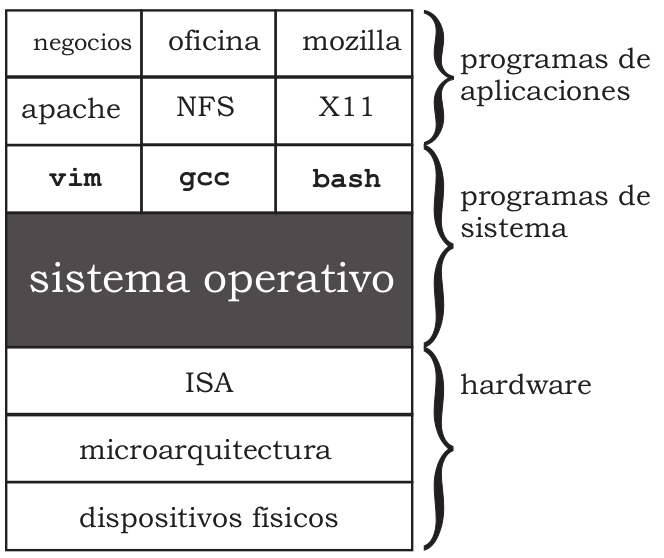
\includegraphics[scale=.50]{./figuras/capas.png}
 % capas.png: 607x522 pixel, 72dpi, 21.41x18.41 cm, bb=0 0 607 522
 \caption{Sistema de cómputo en capas}
 \label{Sistema de cómputo en capas}
\end{figure}


El sistema operativo tiene como misión administrar todos los elementos de un
sistema complejo, por tanto, el sistema operativo efectúa un reparto controlado
de los procesadores, memorias y dispositivos de entrada/salida, entre los
diversos programas que compiten por obtener estos recursos.

El sistema operativo (SO) permite lanzar aplicaciones a través de
procesos\footnote{Proceso, unidad de actividad que se caracteriza por la
ejecución de una secuencia de instrucciones, un estado actual, y un conjunto de
recursos del sistemas asociados\cite{tanenbaum}} o hilos\footnote{Hilo,  es la
unidad de procesamiento más pequeña que puede ser planificada por un sistema
operativo.} y vigilará que los recursos sean utilizados de forma equitativa
entre los procesos.

Para poder realizar estas tareas es necesario tener una jerarquía de ejecución,
esta jerarquía puede establecerse con:

\begin{itemize}

 \item Procesos con privilegos limitados
 \item Procesos con privilegos otorgados temporalmente
 \item Procesos con mayores privilegios
 
\end{itemize}

Para lograr que el sistema operativo logre su objetivo, es necesario que el
procesador tenga al menos dos modos de operación:

\begin{itemize}

 \item Modo \emph{kernel}, o supervisor, permite accesar a todo el
\emph{hardware} y
  permite la ejecución de cualquier instrucción.
 \item Modo usuario, o modo real, solo permite la ejecución de un conjunto
  reducido de instrucciones\cite{nsistemas}.
 
\end{itemize}

\section{Linux}


Linux tiene su origen en Unix, éste apareció en los años sesenta, desarrollado
por los investigadores Dennis Ritchie y Ken Thompson, de los Laboratorios
Telefónicos Bell.

Andrew Tanenbaum desarrolló un sistema operativo parecido a Unix (Minix)
para enseñar a sus alumnos el diseño de un sistema operativo. Debido al enfoque
docente de Minix, Tanenbaum nunca permitió que éste fuera modificado, ya que
podrían introducirse complicaciones en el sistema para sus alumnos.

Un estudiante finlandés llamado Linus Torvalds, constatando que no era posible
extender Minix, decidió escribir su propio sistema operativo compatible con
Unix.

En aquellos momentos el proyecto GNU (\emph{GNU's Not Unix}), que Richard
Stallman había iniciado hacía ya casi diez años, comprendía un sistema básico
casi completo. La excepción más importante era el \emph{kernel} o núcleo, que
controla el \emph{hardware}.

Torvalds decidió aprovechar el sistema GNU y completarlo con su propio núcleo,
que bautizó como Linux (\emph{Linux Is Not UniX}).

El \emph{kernel} es el componente central del sistema operativo. Su funciones
son principalmente administrar el \emph{hardware} de manera coherente y justa
mientras se le otorga un nivel de abstracción familiar, a través de las
APIs\footnote{ API acrónimonimo de \emph{Application Programming Interface}es el
conjunto de funciones y procedimientos que ofrece cierta biblioteca para ser
utilizado por otro software como una capa de abstracción.}, a las
aplicaciones de nivel de usuario.

Entre otras tareas relevantes de un sistema operativo, el \emph{kernel} de Linux
maneja dispositivos, administra los acceso de E/S, controla los procesos y
administra el uso compartido de memoria. Dentro del \emph{kernel}, la interfaz
de bajo nivel es específica para cada configuración de hardware, sobre la cual,
el \emph{kernel} ejecuta y provee control directo de los recursos hardware.

Típicamente, los servicios de bajo nivel manejan operaciones específicas de el
CPU, operaciones de memoria específicas a la arquitectura, y provee interfaces
básicas para dispositivos. Los capa de alto nivel provee abstracciones comunes a
todos los sistemas Unix, incluyendo procesos, archivos, sockets y señales. Este
nivel de abstracción se mantiene constante aunque difiera el hardware.

Entre estos dos niveles de abstracción, el \emph{kernel} necesita lo que se
denomina componentes de interpretación para comprender e interactuar con datos
estructurados provenientes de, o hacia ciertos dispositivos. Los diferentes
tipos de sistemas de archivos y los protocolos de red son ejemplos de fuentes de
datos estructurados. El \emph{kernel} necesita interpretarlos e interactuar a
fin de proveer acceso a los datos provenientes desde estas fuentes o hacia las
mismas.

Los servicios brindados por el \emph{kernel} no son soporte suficiente para
cargar y ejecutar las aplicaciones. Es necesario contar con librerías, éstas
proveen APIs familiares y abstracciones de servicios que interactúan con el
\emph{kernel} en nombre de las aplicaciones para obtener la funcionalidad
deseada.

La librería principal, utilizada en la mayoría de las aplicaciones Linux, es la
librería C GNU (\textbf{glibc}). Típicamente las librerías son enlazadas
dinámicamente en el momento en el que se ejecutan las aplicaciones. Esto es, no
son parte de las aplicaciones binarias, sino que se cargan dentro del espacio de
memoria de las aplicaciones durante el inicio de las mismas. Esto permite a
varias aplicaciones utilizar una misma instancia de una librería en vez de
realizar una copia en memoria por cada aplicación que se ejecuta.

Según lo expuesto anteriormente es lógico pensar la conveniencia de enlazar
dinámicamente las librerías, sin embargo, en los sistemas empotrados esto no es
del todo cierto. El motivo radica en que las aplicaciones no utilizan la
librería C en forma completa, sino que dependiendo de la aplicación puede
utilizar partes de la librería y no otras. De este modo, en algunas aplicaciones
parte de la librería se encuentra en la misma aplicación binaria. Este es el
fundamento por el cual es preferible utilizar un enlazamiento estático, sin
embargo nos encontramos con un inconveniente, para sistemas Linux empotrados la
librería \textbf{glibc} consume demasiados recursos de la memoria RAM del
sistema, por este motivo, reemplazar esta librería puede significar un ahorro de
espacio en memoria. Usualmente se la reemplaza por librerías alternativas
diseñadas para sistemas empotrados.

\subsection{El \emph{kernel} de Linux}

El \emph{kernel} Linux es distribuido bajo la licencia GNU GPL por lo que su
capacidad de evolución es una cualidad que posee desde su surgimiento, hecho por
el cual su desarrollo es muy activo, brindando soporte para cientos de
protocolos de red, decenas de arquitecturas de \emph{hardware} y por supuesto,
obteniendo un rendimiento eficiente y robusto\cite{emiliano}.

Una clasificación generalmente utilizada para clasificar a los sistemas
operativos tiene que ver con el modo de compartir el espacio de memoria. Se
diferencian tres tipos, de tiempo real, monolíticos y microkernel.
De forma resumida las características son las siguientes:

\begin{itemize}
 \item \emph{Realtime}, El espacio de direcciones es plano o lineal, no posee
protección de memoria entre las aplicaciones y el \emph{kernel}, es decir, el
núcleo del \emph{kernel}, el subsitema del \emph{kernel} y las aplicaciones
comparten el mismo espacio de memoria. Se denominan \emph{Realtime} debido a que
no hay sobrecarga por llamadas al sistema, pasaje de mensajes o copia de datos.

   \item Monolítico, está diferenciado el espacio de memoria de usuario y
\emph{kernel}. Las aplicaciones que operan en el espacio de usuario lo hacen
sobre direcciones de memoria virtuales por lo tanto no pueden corromper la
memoria de otras aplicaciones o del \emph{kernel}. Sin embargo, los componentes 
del \emph{kernel} comparten el mismo espacio de direcciones y por ende, un
\emph{drive} o módulo mal programado puede causar la inestabilidad del sistema.
La mayoría de os sistemas operativos Unix son de este tipo.                    
            

  \item Microkernel,  hace uso de un pequeño SO que provee los servicios básicos
y el resto del \emph{kernel} se ejecuta como aplicaciones. La clave del
microkernel surge a partir de un esquema robusto de paso de mensajes.

\end{itemize}

Cuando un programa es ejecutado en modo usuario este no puede acceder
directamente a programas o estructuras de datos del \emph{kernel}, sin embargo,
cuando el mismo se ejecuta en modo \emph{kernel} estas restricciones no existen.


\subsection{Sistema de archivos}

El sistema de archivos es el encargado de realizar la organización y
almacenamiento de los archivos en los diferentes dispositivos disponibles en el
sistema. En función de las características del dispositivo de almacenamiento y
del tipo de información que se va a guardar es preferible utilizar un sistema de
archivos u otro.

Linux da soporte a varios sitemas de archivos, dentro de los más utilizados se
encuentran ext2, ext3, etc. Estos sistemas de archivos son manejados
por una capa denominada Sistema de Archivos Virtual (VFS\footnote{VFS, es una
capa de abstracción encima de un sistema de archivos más concreto. El propósito
de un VFS es permitir que las aplicaciones cliente tengan acceso a diversos
tipos de sistemas de archivos concretos de una manera uniforme. Puede ser
utilizada para tender un puente sobre las diferencias en los sistemas de
archivos de Windows, de Mac OS y Unix, de modo que las aplicaciones pudieran
tener acceso a archivos en los sistemas de archivos locales de esos tipos sin
tener que saber a qué tipo de sistema de archivos están teniendo acceso.}). Esta
capa de abstracción provee una visión consistente de los datos almacenados en
diferentes dispositivos del sistema. Esta visión es lograda separando el nivel
de usuario de los sistemas de archivos, utilizando llamadas estándar al
sistema, permitiendo sistemas de archivos lógicos sobre cualquier dispositivo
físico. Por lo tanto esta capa abstrae los detalles físico del dispositivo
permitiendo un acceso a los mismos a través de archivos de una maner
consistente.

Por debajo de esta capa VFS, el \emph{kernel} interactúa con dispositivos de E/S
a través de controladores de dispositivos. Estos controladores se encuentran
incluidos en el \emph{kernel} y consisten en estructuras de datos y funciones
que controlan uno o más dispositivos como discos rígidos, teclados, mouses,
monitores, interfaces de red, dispositivos SCSI.

Uno de los propósitos fundamentales de los controladores de dispositivos es
aislar los programas de usuario del acceso a estructuras de datos críticas del
\emph{kernel} y dispositivos de \emph{hardware}. Además, un controlador de
dispositivo oculta al usuario la complejidad y variabilidad de un dispositivo
\emph{hardware}. Por ejemplo, un programa que quiere escribir datos en un disco
rígido no tiene en cuenta si el mismo posee sectores de 512 bytes o 1024 bytes.
El usuario simplemente abre el archivo y realiza el comando de escritura. El
controlador manejará los detalles y aislará al usuario de las complejidades y
riesgos de programar directamente sobre el dispositivo de \emph{hardware}. Estos
controladores proveen la representación de los dispositivos a través de
archivos, en GNU/Linux y sistemas operativos Unix todo \emph{hardware} es
representado por un archivo.

Linux posee la capacidad de agregar y quitar componentes del \emph{kernel} en
tiempo de ejecución. Como hemos descrito anteriormente, el \emph{kernel} Linux
posee una estructura de \emph{kernel} monolítico, con una interfaz para agregar
y quitar módulos de controladores de dispositivos dinámicamente luego del
arranque del mismo. Esta característica no solo agrega flexibilidad al usuario,
sino que además, en sistemas empotrados adquiere una especial importancia debido
a su capacidad de actualización y adaptación a dispositivos de E/S
nuevos\cite{understanding}.

Todo dispositivo, ya sea que se encuentre en un sistema empotrado o una PC de
escritorio, necesita al menos un sistema de archivos. La principales razones de
esto son:

\begin{itemize}
 \item Las aplicaciones poseen programas separados, independientes por ende
necesitan espacio de almacenamiento en un sistema de archivos.
 \item Los dispositivos de bajo nivel también son accedidos mediante archivos.
\end{itemize}

\section{\emph{Embedded Linux}}

Linux empotrado, del inglés: \emph{Embedded Linux} se refiere al uso de un
sistema operativo basado en Linux en un sistema empotrado, como por ejemplo
teléfonos móviles, robots, servidores, dispositivos electrónicos y aplicaciones
industriales con microcontroladores y microprocesadores\cite{embedded}.

Para implementar un sistema Linux empotrado en un dispositivo de
\emph{hardware}, se debe conocer en términos generales la arquitectura del
mismo, es decir, el tipo de micro-procesador que posee, la cantidad de memoria,
los buses que soporta, los componentes que posee la tarjeta de desarrollo,
etc. Esta información es de vital importancia, ya que al preparar el sistema
Linux que se ejecutará en el dispositivo, se debe compilar con soporte
para esas características. La tarea de construir un sistema operativo
basado en Linux que se ejecute en este dispositivo objetivo se debe
realizar mediante compilación cruzada.

\subsection{¿Por qué \emph{Embedded Linux}?}
 
\subsubsection{Independiencia de Proveedores}

Selecionar un sistema operativo propietario para la construcción de este
proyecto podría limtar la vida útil del mismo, la falta de  soporte por parte
del proveedor resultaría en mayor tiempo de desarrollo, \emph{Embedded Linux}
es un sistema operativo independiente el cual comparte muchas caraceristícas
con sistemas operativos propietarios como puden ser el \emph{kernel},
librerias, utilidades básicas, etc.

\subsubsection{Variedad de \emph{hardware} soportado}

Debido al crecimiento exponencial de componentes para sistemas embebidos las
dificultades para dar soporte a todos estos componentes a  aumentado
considerablemente,\emph{Embedded Linux} soporta multiples arquitecturas y
dispositivos de entrada y salida, además es aceptado en univeridades como una
herramienta de desarrollo e investigación lo que ayuda  a mantener una gran
variedad de \emph{hardware} soportado por el \emph{kernel}.

\subsubsection{Bajo Costo}

\emph{Embedded Linux} conlleva bajos costos en su desarrollo , capacitación y
mantenimiento, además todas las herramientas como compiladores, \emph{linkers},
librerias, \emph{shells} pueden ser descargadas a través de internet de forma
libre,

\subsection{\emph{Open Source}}

Una de las principales razones por las que Linux es tan popular es que es de
código abierto, Linux tiene  ventajas del \emph{Open
Source}\cite{raghavan2005embedded} como:
\begin{itemize}
 \item Hay miles de desarrolladores contibuyendo a la mejora continua del
 \emph{kernel} de Linux y otras aplicaciones.
 \item Asegura un soprte global durante el proceso de desarrollo.
 \item Amplia disponibilidad de código  y controladores de dispositivos de
 \emph{hadware}.
 \item Las aplicaciones y utilidades integradas con Linux tienen una naturaleza
\emph{Open Source}, teniendo todos los beneficios antes mencionados. 
\end{itemize}















